
\chapter{Glassy Patterns\label{ch:glass}}

\graphicspath{{ch-glass/figures/}}

\section{Introduction}

Molecular systems often have complicated trajectories that cannot be analyzed by simple statistical techniques. Diffusion maps are one method of analysis to extract relevant features of the molecular dynamics. As a model system, I looked at a cluster of 7 Lennard-Jones particles in two dimensions. These are point particles that have a pairwise interaction potential given by
\begin{equation}
\label{LJ}
V_{LJ}=\epsilon\left\{\left(\frac{r^{*}}{r}\right)^{12}-2\left(\frac{r^{*}}{r}\right)^{6}\right\}
\end{equation}
where $r$ is the interparticle distance, $r^{*}$ is the minimum in the interaction potential, and $\epsilon$ is the depth of the potential well.\footnote{Terrell L. Hill, \underline{An Introduction to Statistical Thermodynamics}, Dover Publications, 1986, pp. 484-485} 

I used molecular dynamics to simulate this cluster at constant energy. Molecular dynamics integrates the equations of motion beginning from some initial configuration. At each time step, the forces on each particle are calculated from the Lennard-Jones potential; the acceleration, $\mathbf{a}$, of each particle can then be calculated from the forces, and new positions, $\mathbf{x}$, and velocities, $\mathbf{v}$, can then be calculated since $\mathbf{a}=\frac{d\mathbf{v}}{dt}$ and $\mathbf{v}=\frac{d\mathbf{x}}{dt}$. I then analyzed the configurations obtained from the molecular dynamics simulations using diffusion maps. 

\section{Comparing configurations}
Using diffusion maps to analyze particle trajectories requires a distance measure for comparing pairs of particle configurations. The simplest method is to construct a set of features that contains all the information relevant to a particular configuration, and then compare features. Because I looked at clusters of identical particles, I required features that are invariant to permutations of particle labels, as well as translations and rotations. I first mean-centered each configuration, to remove any translational degrees of freedom. I treated the particle coordinates as points in the complex plane, so each particle was represented as
\begin{equation}
z_j=r_{j}e^{i\theta_j} \ \ j=1,\dots,7
\end{equation}

Define complex moments as follows:
\begin{equation}
c_{pq}=\sum_{j=1}^{7}z_{j}^{p}\overline{z_{j}}^{q}=\sum_{j=1}^{7}\left(r_{j}e^{i\theta_j}\right)^{p}\left(r_{j}e^{-i\theta_j}\right)^{q}=\sum_{j=1}^{7}r_{j}^{p+q}e^{i(p-q)\theta_j}
\end{equation}
where $\overline{z_j}$ denotes conjugation. The $c_{pq}$ is permutation-invariant, since it is symmetric polynomial.

To make the features rotation invariant, note that, if a configuration is rotated by phase $\alpha$, then the new moment, $\hat{c_{pq}}$, can be written as
\begin{equation}
\hat{c_{pq}}=\sum_{j=1}^{7}r_{j}e^{i(p-q)(\theta_j+\alpha)}=e^{i(p-q)\alpha}\sum_{j=1}^{7}r_{j}e^{i(p-q)\theta_j}=e^{i(p-q)\alpha}c_{pq}
\end{equation}

Therefore, consider products of moments
\begin{equation}
\prod_{i=1}^{n}c_{p_{i}q_{i}}^{k_i}
\end{equation}
such that 
\begin{equation}
\sum_{i=1}^{n}k_i(p_i-q_i)=0
\end{equation}
These products will be rotationally invariant.

The following independent rotationally-invariant quantities were proposed by Flusser \footnote{Jan Flusser, ``On the independence of rotation moment invariants,'' \underline{The Journal of the Pattern Recognition Society}, Vol. 33, pp. 1405-1410}:
\begin{itemize}
\item $x_1=c_{11}$
\item $x_2=c_{12}c_{21}$
\item $x_3=c_{20}c_{12}^2$
\item $x_4=c_{30}c_{12}^3$
\item $x_5=c_{22}$
\item $x_6=c_{31}c_{12}^2$
\item $x_7=c_{40}c_{12}^{4}$
\end{itemize}
Flusser suggests comparing the real and complex parts of each $x_{j}$ as a method of comparing two sets of points.

However, since each $x_{j}$ contains a different power of $r$, the moments must be appropriately normalized so that they can be accurately compared. If $x_{j}=r_{j}e^{i\theta_{j}}$, and if $x_{j}$ is the sum of terms of the form $r^{n}e^{i\theta}$, then appropriate moments would be $\psi_{j}=r_{j}^{1/n}e^{i\theta_j}$. Therefore, define the following normalized moments:
\begin{itemize}
\item $\psi_1=x_1^{1/2}$
\item $\psi_2=x_2^{1/6}$
\item $\psi_3=Re(|x_3|^{-7/8}x_{3})$
\item $\psi_4=Im(|x_3|^{-7/8}x_{3})$
\item $\psi_5=Re(|x_4|^{-11/12}x_{4})$
\item $\psi_6=Im(|x_4|^{-11/12}x_{4})$
\item $\psi_7=x_5^{1/4}$
\item $\psi_8=Re(|x_6|^{-9/10}x_{6})$
\item $\psi_9=Im(|x_6|^{-9/10}x_{6})$
\item $\psi_{10}=Re(|x_7|^{-15/16}x_{7})$
\item $\psi_{11}=Im(|x_7|^{-15/16}x_{7})$
\end{itemize}

The original system has 14 degrees of freedom (2 coordinates for each of the 7 particles). When removing the 2 translational degrees of freedom and the 1 rotational degree of freedom, there are 11 remaining degrees of freedom. Therefore, using the 11 independent moments $\psi_1,\dots,\psi_{11}$ should determine the system.

After computing $\psi_1,\dots,\psi_{11}$ for each configuration, distance between pairs of configurations can be calculated as
$$d^2_{ij}=\sum_{k=1}^{11}\frac{\left(\psi_{k}(i)-\psi_{k}(j)\right)^{2}}{\sigma_k}$$
where $\sigma_k$ is an additional weighting factor that is a measure of the noise of the moment. Some moments are more sensitive to noise than others, and should therefore contribute less to the overall distance. 

I chose $\sigma_k$ to be the average ``local'' variance, under the assumption that in a trajectory, neighboring trajectories are most likely similar and any variations are due to noise. So, take $\delta$ to be the number of points to use in the average (the following analysis used $\delta=3$), then
$$\sigma_k=\frac{1}{n-\delta}\sum_{i=1}^{n-\delta}\left(\frac{1}{\delta}\sum_{j=i}^{i+\delta}(\psi_{k}(j)-\overline{\psi_{k}})^{2}\right)$$
where $\overline{\psi_{k}}$ is the average $\psi_{k}$ taken over configurations $i, i+1,\dots,i+\delta$. 

\section{Diffusion Maps}
I then used diffusion maps to analyze the system dynamics. The original trajectory consisted of 50,000 configurations. Due to computational resources, I used every third configuration in the analysis. I constructed the weight matrix $W$, with
$$W_{ij}=exp\left(-\frac{d_{ij}^2}{\sqrt{\epsilon}}\right)$$
where $\epsilon$ is the kernel width (chose $\epsilon=25$). 

Define the diagonal matrix $D$ with
$$D_{ii}=\sum_{j=1}^{n}W_{ij}$$
and the random walk matrix $A$ as
$$A=D^{-1}W$$

Then the diffusion map is given by the eigenvectors of $A$, $\phi_{1},\dots,\phi_{n}$, where configuration $i$ is mapped to the point $(\phi_{1}(i),\phi_{2}(i),\dots,\phi_{n}(i))$.

\section{Results}

\subsection{Diffusion Map Embedding}

\begin{figure}[t]
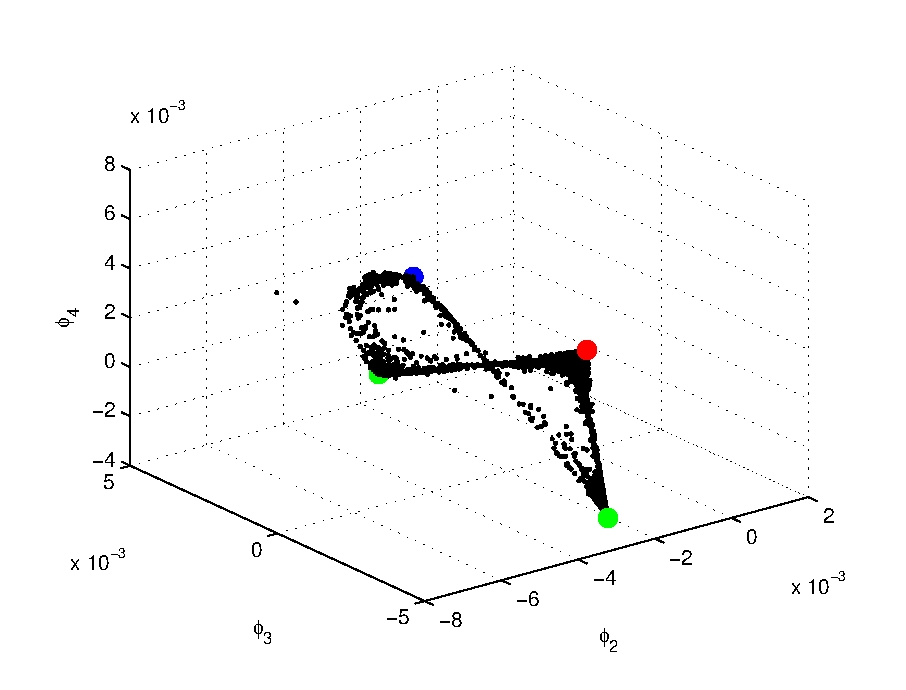
\includegraphics[width=11cm]{dmap}
\caption[Diffusion maps embedding of Lennard-Jones cluster]{The diffusion map embedding of the configurations}
\label{dmap}
\end{figure}

\begin{figure}[t]
\begin{subfigure}{7cm}
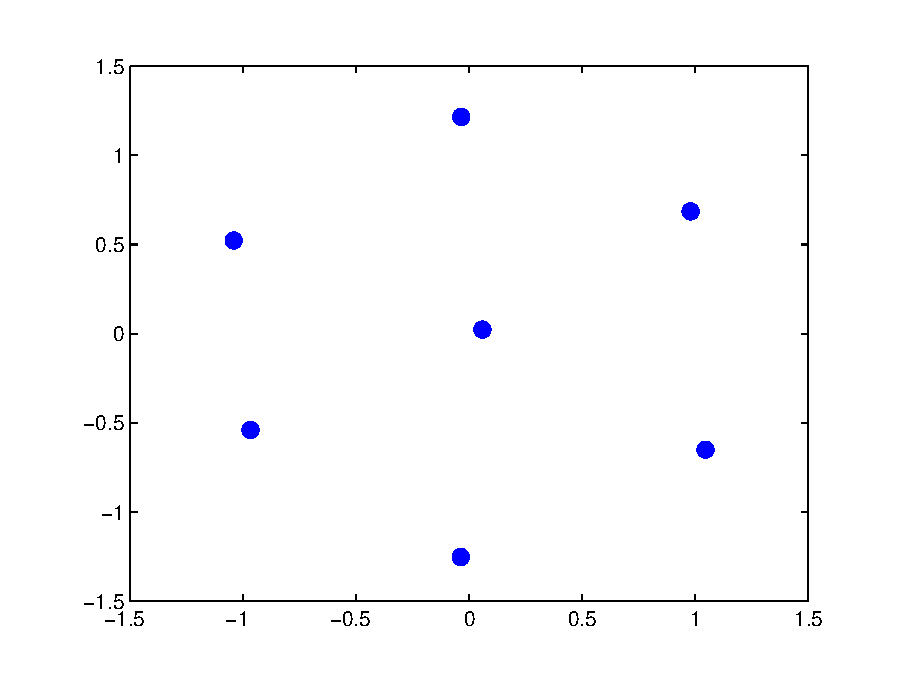
\includegraphics[width=\textwidth]{config1}
\end{subfigure}
%
\begin{subfigure}{7cm}
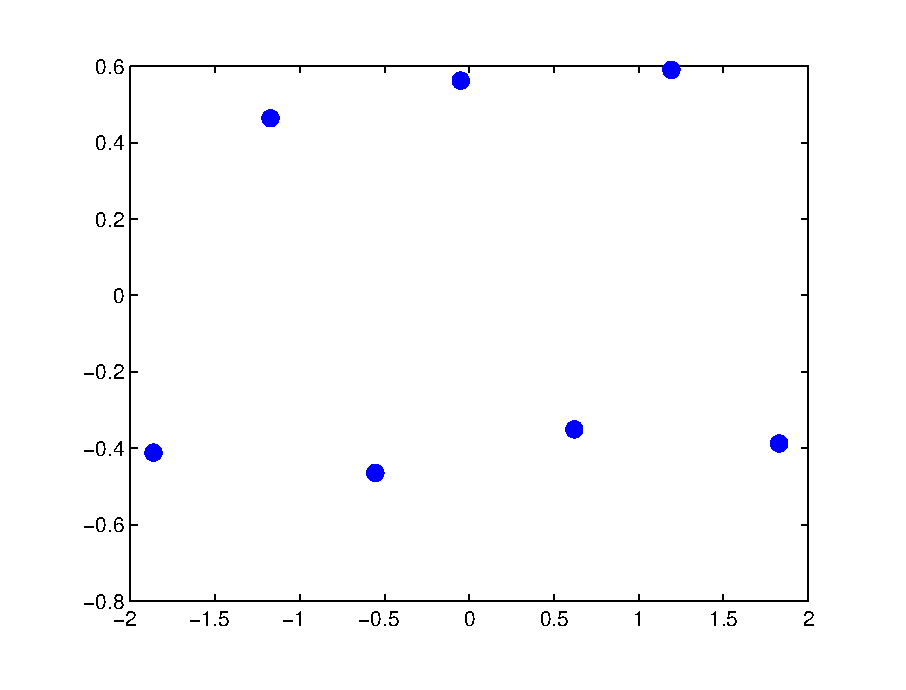
\includegraphics[width=\textwidth]{config4}
\end{subfigure}

\begin{subfigure}{7cm}
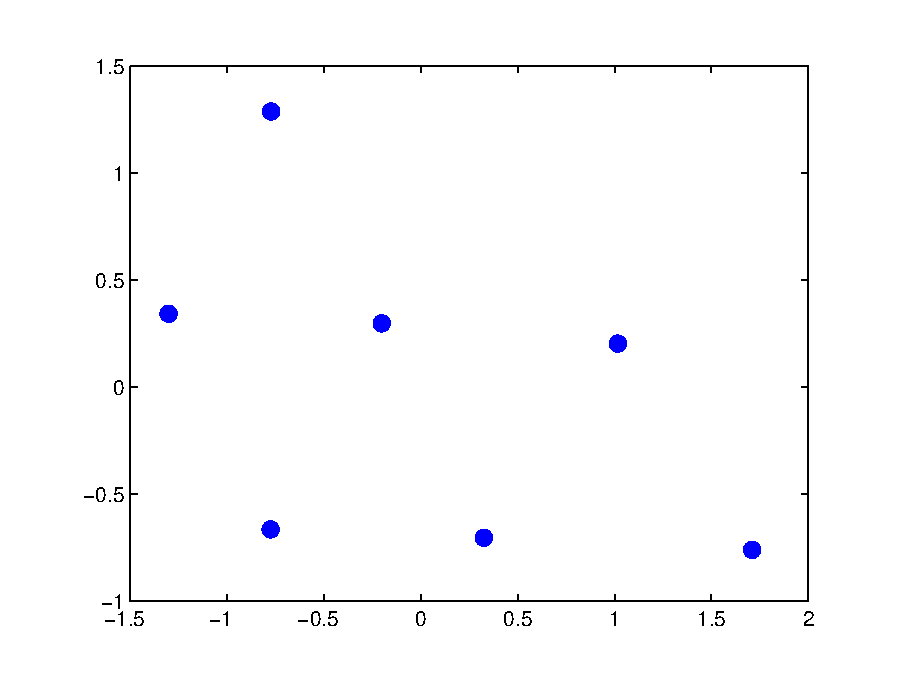
\includegraphics[width=\textwidth]{config2}
\end{subfigure}
%
\begin{subfigure}{7cm}
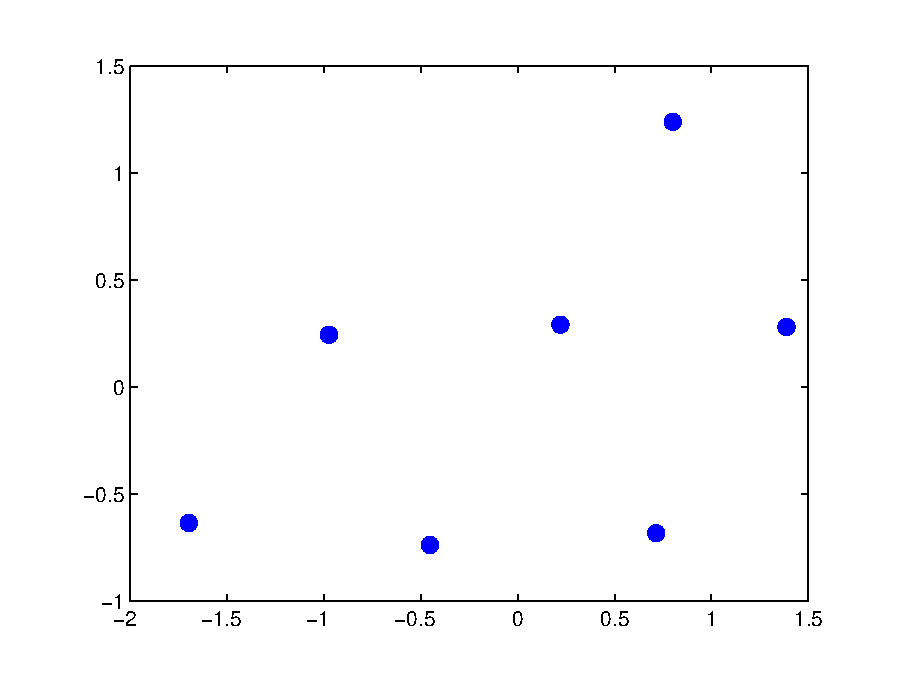
\includegraphics[width=\textwidth]{config3}
\end{subfigure}
\caption[Representative configurations of Lennard-Jones cluster]{Configurations corresponding to the red point (a), blue point (b), and the two green points (c,d) in Figure \ref{dmap} and \ref{dmap_noreflec}}
\label{fig2}
\end{figure}

\begin{figure}[t]
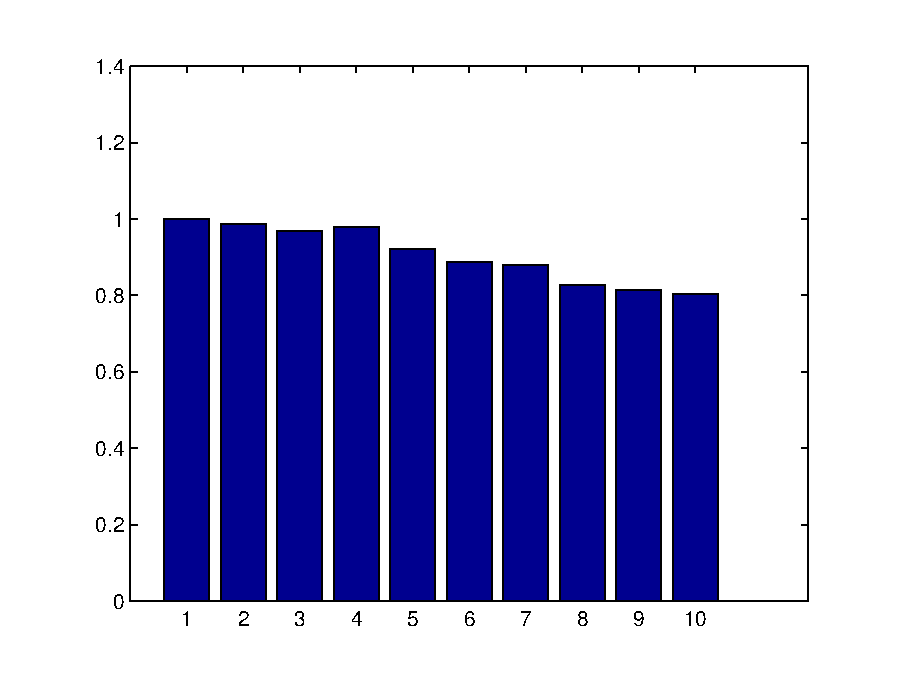
\includegraphics[width=8cm]{evals.eps}
\caption[Eigenvalue spectrum for diffusion maps embedding of Lennard-Jones cluster]{Plot of the top 10 eigenvalues from the diffusion map embedding}
\label{evals}
\end{figure}

Figure \ref{dmap} shows the embedding of the particle configurations into the first 3 nontrivial eigenvectors of $A$. There are 4 distinct clusters of points, with transition paths connecting them. Figure \ref{fig2} shows the configurations corresponding to the colored points. The two green points in Figure \ref{dmap} correspond to configurations that are reflections of each other. This is consistent with the diffusion map embedding, which exhibits symmetry about the $\phi_3=0$ plane. Also, the diffusion map shows that there is no direct transition from configuration (a) to configuration (b). All transitions must first visit configuration (c) or (d). Please note that the blue-green and red-green paths in Figure \ref{dmap} do not cross. An overlap would correspond to the intermediate configuration  between the green and blue points becoming symmetric. Also, in Figure \ref{evals}, you see the top 10 eigenvalues for the diffusion map embedding. Eigenvectors 2, 3, and 4 were used for the embedding in Figure \ref{dmap}, although the coordinates were not scaled by the corresponding eigenvalues. 

\subsection{Reflection-Invariant Features}

As Flusser states, using only the real parts of the rotation-invariant moments will result in reflection-invariant moments. Therefore, I used $\psi_1,\psi_2, \psi_3,\psi_5,\psi_7,\psi_8,$ and $\psi_{10}$ to compute the reflection-invariant diffusion map.

Note that the original system has 14 degrees of freedom, and removing the 2 translational, 1 rotational, and 1 refective degrees of freedom leaves 10 degrees of freedom. Therefore, the 7 refelction-invariant moments defined above do not uniquely determine the configuration. 

\begin{figure}[t]
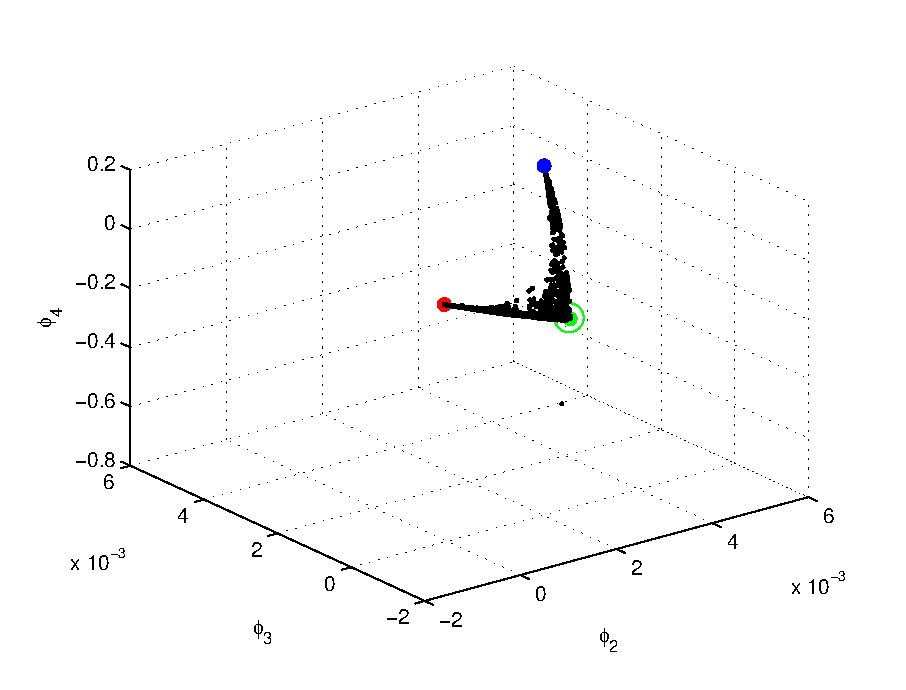
\includegraphics[width=11cm]{dmap_noreflec.eps}
\caption[Diffusion maps embedding of Lennard-Jones cluster using rotation-invariant moments]{Diffusion map embedding from using the moments defined in \ref{mom_list}; the green point and green circle correspond to the two green points in Figure \ref{dmap}}
\label{dmap_noreflec}
\end{figure}

As you can see, in Figure \ref{dmap_noreflec}, the two green points in Figure \ref{dmap} collapse into one point. From Figure \ref{fig2}, we can see that the two green points correspond to mirror image configurations. Therefore, removing the imaginary moments removed the reflective degrees of freedom, as expected. 

\subsection{Comparison of Diffusion Maps with Principal Components Analysis}
Using all 11 moments, Principal Components Analysis (PCA) was performed. As seen in Figure \ref{PCA}, no significant structure is uncovered using PCA.
\begin{figure}[t]
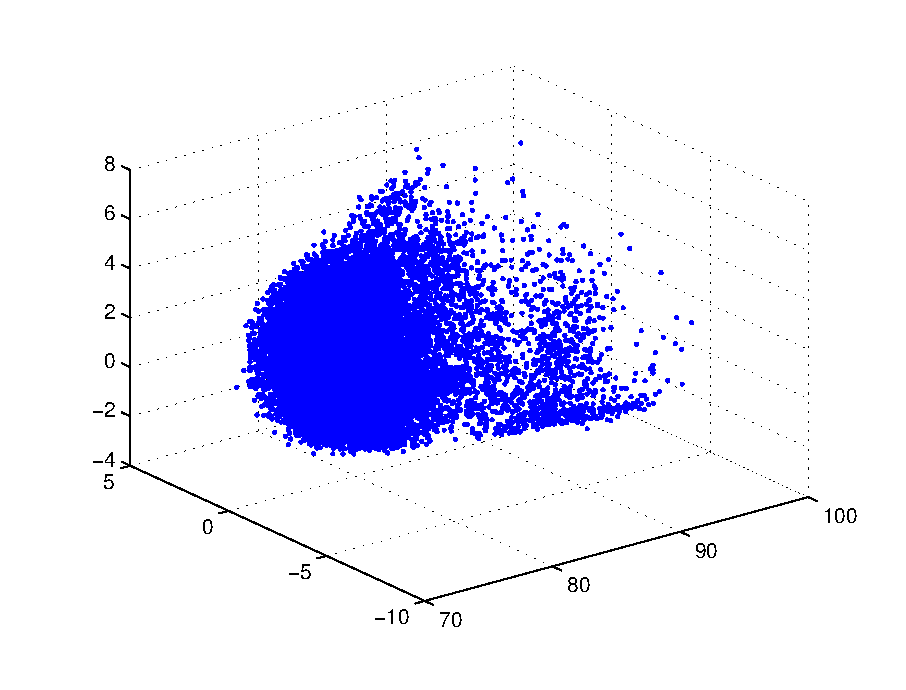
\includegraphics[width=8cm]{PCA.eps}
\caption[Principal components embedding of Lennard-Jones cluster]{The projection of the data onto the first 3 principal components}
\label{PCA}
\end{figure}

\subsection{Definition of $\sigma$}
The use of weighting factors in the distance computation proved important for the use of diffusion maps. As seen in Figure \ref{dmap_nosigma}, removing the weighting factors significantly distorts the embedding. The transition pathways are much clearer in the embedding in Figure \ref{dmap}.

\begin{figure}[t]
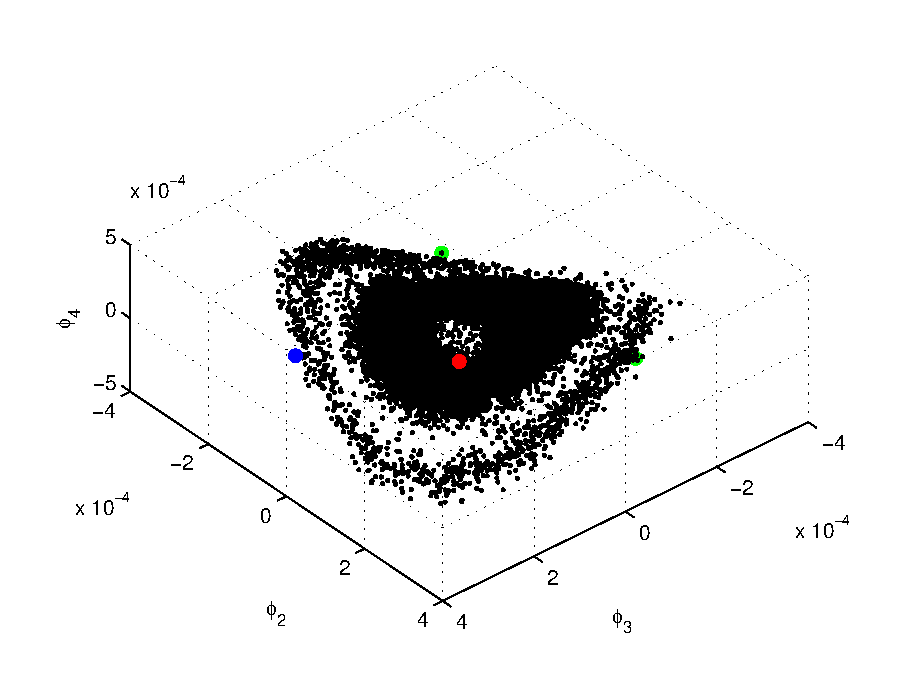
\includegraphics[width=10cm]{dmap_nosigma.eps}
\caption[Diffusion maps embedding of Lennard-Jones cluster without weight factors]{The diffusion map embedding of the configurations without the weighting factors $\sigma_k$ in the distance definition; the colored points correspond to the configurations in Figure \ref{fig2}}
\label{dmap_nosigma}
\end{figure}

\section{Conclusion}
I used diffusion maps to analyze the dynamics of a cluster of 7 Lennard-Jones particles. I established a distance measure between particle configurations that was invariant to translations, rotations, and permutations of particle labels. I then used diffusion maps to conclude that there are several meta-stable configurations of the particles, and there are different transition pathways between the different configurations. Future work would include further refining the distance measure between configurations to make it more accurate, as well as doing this analysis for a longer simulation to perhaps extract more features of the particle dynamics.